\subsection{FindBugs}
FindBugs was used for static analysis of Java code as the first step in finding vulnerablities in the Smart Card Simulator.

\subsubsection{InternetBanking}
FindBugs reported 3 issues in the Java code of InternetBanking, out of which 1 was categorized as \code{High confidence} and the other 2 as \code{Low confidence}. See \ref{fig:findbugs_overview} for the scan report.
The issues are mostly related to coding practices \& conventions and are listed below, while one of them could be of concern.
\begin{itemize}
	\item Use of default encoding instead of specifying an explicit character encoding when converting to bytes
	\item Catch of an unthrown exception
	\item Call to swing method outside the swing thread
\end{itemize}
As seen, they are easy to correct and do not require much time or effort. The last one refers to the invocation of the \code{pack} function. The Swing methods \code{pack()} will create the associated peer for the frame. This causes the system to create the event dispatch thread. This makes things problematic because the event dispatch thread could be notifying listeners while pack and validate are still processing. This situation could result in two threads going through the Swing component-based GUI. This s a serious flaw that could result in deadlocks or other related threading issues.

\subsubsection{SecureBank}
FindBugs reported 9 issues in the Java code of SecureBank, out of which 1 was categorized as \code{Troubling}. See \ref{fig:findbugs_overview_secure_bank} for the scan report.
The issue was about a possible null pointer dereference on exception path. Upon analyzing the code, it was found that the variable can be null only if an excpetion is thrown while trying to get an instance of \code{MessageDigest}, which is an issue, though very rare. However, this does not lead to any security problems.
The other issues are related to coding practices \& conventions and are listed below.
\begin{itemize}
	\item Use of == or != instead of equals to compare strings
	\item Use of platform default encoding instead of specifying an explicit character encoding when opening a file
	\item Redundant null check of a variable, which is known to be non-null
	\item Use of non-localized \code{String.toUpperCase()} or \code{String.toLowerCase()}
\end{itemize}
As seen, they are easy to correct and do not require much time or effort. The last one is not relevant as the application does not support Internationalization.

\begin{figure}[ht]
	\centering
	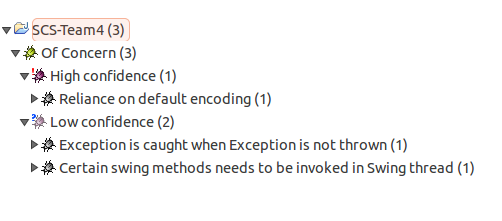
\includegraphics[width=.8\linewidth]{figures/findbugs_overview.png}
	\caption{Overview of FindBugs scan for InternetBanking}
	\label{fig:findbugs_overview}
\end{figure}

\begin{figure}[ht]
	\centering
	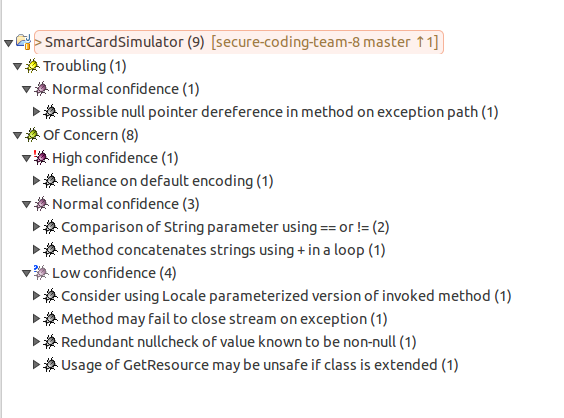
\includegraphics[width=.8\linewidth]{figures/findbugs_overview_secure_bank.png}
	\caption{Overview of FindBugs scan for SecureBank}
	\label{fig:findbugs_overview_secure_bank}
\end{figure}